\chapter{Erhebung der Anforderungen an das neue Korrelationsformat}\label{ch:anforderungen}


\section{Methode zu Erhebung der Anforderungen}

Zur Herleitung der Anforderungen an das neue Korrelationssystem wird zunächst die interne Produkterfassung der \metaeffektsp beschrieben, die in den meisten Fällen als Ausgangspunkt der Produktidentifikation dienen wird.
Aus diesem werden die unterschiedlichen relevanten Software-Ökosysteme vorgestellt und wie sich diese in den Software-Inventaren darstellen.
Das bestehende Korrelationsformat wird anschließend auf seine Schwächen und Herausforderungen untersucht, woraus die Anforderungen an das neue Korrelationsformat abgeleitet werden.
Der Ausgangspunkt der Herausforderungssuche ist das ursprüngliche Problem, aufgrund dessen das bestehende Korrelationsformat entwickelt wurde:
Der Mangel an präzisen Daten in den verwendeten Datenquellen und den fehlenden Verknüpfungen zwischen diesen fordert eine Kuration von Abbildungen, die sich allerdings nur aufwendig automatisiert oder manuell herstellen lassen.


\section{Interne Produktmodellierung der \metaeffektlg}\label{sec:metaeffekt-inventory-format}

Wie alle Datentypen im Inventar basieren auch Artefakte auf Key-Value-Pairs, einer frei definierbaren Zuordnung von Textschlüsseln zu Textwerten.
Dieses Format wurde gewählt, um möglichst einfach Änderungen und neue Felder einführen zu können, ohne Schemata definieren und ändern zu müssen.
Komplexere Werte als flache Texte werden z.\ B.\ automatisch als JSON-Objekte serialisiert und beim Einlesen wieder als Objekte deserialisiert.

Für Artefakte ist die zugrundeliegende Struktur mit einigen Basis-Feldern für alle Software-Ökosysteme die gleiche, jedoch unterscheidet sich je nach Ökosystem die tatsächliche Verwendung der Felder.
Jedes Ökosystem hat somit eine übliche Menge an Feldern, mit denen eine Komponente beschrieben wird, die typischerweise ausgefüllt werden.

% FIXME: Why does this table reference not resolve in the document?
Beispielhafte Artefakte aus dem Java/Maven-Ökosystem sind in \autoref{tab:inventory-artifact-entries} dargestellt.

\begin{table}[ht]
    \centering
    \begin{tabular}{llll}
        \toprule
        \textbf{Id}                  & \textbf{Component}         & \textbf{Group Id}        & \textbf{Version} \\
        \midrule
        commons-codec-1.15.jar       & Apache Commons Codec       & commons-codec            & 1.15             \\
        commons-collections4-4.1.jar & Apache Commons Collections & org.apache.commons       & 4.1              \\
        slf4j-api-1.7.36.jar         & SLF4J                      & org.slf4j                & 1.7.36           \\
        log4j-api-2.14.0.jar         & Apache Log4j               & org.apache.logging.log4j & 2.14.0           \\
        \bottomrule
    \end{tabular}
    \caption{Beispielhafte Artefakteinträge in einem Software-Inventar}
    \label{tab:inventory-artifact-entries}
\end{table}

Die \texttt{Id} eines Artefakts ist das einzige Attribut, welches auf einem Artefakt immer gesetzt sein muss.
Sie ist meist einfach der Dateiname, wie er im Dateisystem vorgefunden wurde, inklusive Versionen und Dateiendungen.

Da das Datenmodell tabellarisch angeordnet ist und damit in Tabelleneditoren mit mehreren Tabellenblättern abbildbar ist, wird es häufig in menschenlesbarer Form als \texttt{.xlsx} oder ähnlichen Formaten exportiert.

\subsection{Analyse bestehender Softwareinventare}\label{subsec:analysis-ae-software-inventories}

Da die Darstellungsweisen von Artefakten unterschiedlicher Software-Ökosysteme in den \metaeffekt-Software-Inventaren nicht vollständig normiert sind, wurde ein Datensatz mit den Artefakten aus 1820 realen Software-Inventaren von unterschiedlichen Quellen in einer Datenbank aggregiert und auf Muster untersucht.
% Component Source Type --> Specific Type
Es stellt sich heraus, dass in den meisten Fällen die Art eines Artefakts durch eine Kombination von drei Attributen ableiten lässt: \texttt{Type}, \texttt{Specific Type} und \texttt{Ecosystem}.
Nicht immer sind alle gesetzt, und manchmal kommt es auf die Kombination mehrerer an.

Das Attribut \texttt{Ecosystem} in Artefakten entspricht dem \texttt{type}-Attribut in \acrshortpl{purl} und kann von den erzeugenden Prozessen nur dann aufgefüllt werden, wenn auch eine \acrshort{purl} angegeben ist.
Fehlt dieses, kann meist \texttt{Specific Type} für eine allgemeine Klassifikation und \texttt{Type} für die spezifischere Einordnung in ein zweistufiges hierarchisches Modell verwendet werden.
Leider wurden in dem Datensatz oft Artefakte komplett ohne Typ-Information gefunden, in diesen Fällen müssen weitere Algorithmen zur Erkennung etwa basierend auf Dateiendungen oder anderen Attributen entwickelt werden.

Ein Auszug aus den Werten des \texttt{Ecosystem}-Attributs:
\texttt{npm}, \texttt{gem}, \texttt{github}, \texttt{cpan}, \texttt{wut}, \texttt{docker}, \texttt{conan}, \texttt{deb}, \texttt{nuget}, \texttt{generic}, \texttt{maven}, \texttt{rpm}, \texttt{pypi}, \texttt{golang}, \texttt{apk}.

Die beobachteten Werte aus den Attributen \texttt{Specific Type} und \texttt{Type} reichen von Ökosystemen und Dateitypen bis hin zu Begriffen aus der Betriebssystem- und Gerätetreiberdomäne.
Da sich einige Typen in unterschiedlichen Schreibweisen oder Bedeutungen wiederholen, kann von einer stark heterogenen Entstehung der Artefakte ausgegangen werden.
Die folgenden Kombinationen aus \texttt{Type} → \texttt{Specific Type} konnten im Datensatz gefunden werden:

\begin{itemize}
    \itemsep0em

    \item \texttt{package → generic-version, java-runtime, <empty>}
    \item \texttt{web-module → pwa-module, bower-module, npm-module, <empty>}
    \item \texttt{nodejs-module → npm-module, <empty>} (Alte Schreibweise, kommt so nur in legacy-Inventaren vor)
    \item \texttt{module → jar-module}
    % FIXME-KKL: review
    %  was genau sollte ich hier reviewen?
    \item \texttt{package, python-module, nodejs-module, bios, file → <empty>}
    \item \texttt{operating system → <empty>}
    \item \texttt{(hardware/drivers) storage controller, imaging hardware, operating-system, audio hardware, power driver, mouse, Universal Serial Bus controller driver, data storage, multimedia output device, device connector, firmware driver, storage driver, printer driver, power supply, extension module, disk drives driver, printer, input device, audio driver, computer driver, display driver, processing core, driver, sensor, multimedia driver, appliance, security token, sound hardware, network driver, mouse driver, usb controller driver, security device driver, Bluetooth driver, keyboard, controller, operating system, display, imaging driver, port driver, security hardware, input device driver, system device driver, keyboard driver, print queue driver, processor driver, software device driver, networking hardware, board → <empty>}
    \item \texttt{<empty>}
\end{itemize}

Bei einer Sichtung des Quellcodes einiger Entstehungsquellen von Artefakten konnte die große Auflistung der Hardware- und Betriebssystemtypen in dem Windows-Inventar-Extraktor System gefunden werden, die restlichen sind über diverse Extraktoren verteilt oder werden extern aufgefüllt und damit nicht einheitlich.

\subsection{Erkennungsrichtlinien für unterschiedliche Ökosysteme}\label{subsec:erkennung-typspezifische-artefakte}
% TODO: erkennungsrichtlinien für einzelne ökosysteme



\section{Aktuelles Korrelationsformat zur Modifikation von Artefaktmetadaten}\label{sec:current-correlation-format}

Das Korrelationsformat wurde 2021 entwickelt, um manuelle Nachkorrekturen an den durch die \enquote{CPE Derivation} automatisch abgeleiteten \acrshort{cpe}-Identifikatoren zu ermöglichen.
Während der Hauptanwendungsfall daraus besteht, fehlerhafte oder unpassende \acrshort{cpe}-Zuordnungen zu korrigieren, ermöglicht es die Modifikation beliebiger Artefaktattribute, und wurde so über die Zeit für viele weitere Anwendungsfälle eingesetzt.

Das Format basiert auf \acrfull{yaml} und folgt einem zweistufigen Modell:
Über einen Selektor werden Regeln für die Auswahl von Artefakten definiert, und dann eine Reihe an Modifikationen, die an diesem Artefakt vorgenommen werden sollen.
Jeder Korrelationseintrag kann aus den folgenden Attributen bestehen, wobei mindestens ein \texttt{affects} und eine Modifikationsoperation definiert sein muss.
Ein kleines Beispiel bei dem eine \acrshort{cpe} zu einem Artefakt hinzugefügt wird kann in \autoref{lst:correlation-initial-example} gefunden werden, ausführlichere Beispiele mit Beschreibungen werden nach der Formatbeschreibung aufgeführt.

\begin{lstlisting}[style=yaml,caption={Korrelationseintrag für die Java-Komponente Liquibase},label={lst:correlation-initial-example}]
- affects:
    - Id: liquibase-*.jar
    - Id: org.liquibase.liquibase-*.jar
  append:
    Additional CPE URIs: cpe:/a:liquibase:liquibase
\end{lstlisting}

\paragraph{Artefakt-Selektion}
Die \texttt{affects}-Sektion eines Eintrages muss immer vorhanden sein und legt fest, auf welche Artefakte sich der Eintrag beziehen soll.
Dabei wird in einer Listenstruktur eine Menge an Attribut-Wert-Paaren angegeben, die auf der Ebene der Liste logisch als ODER-Verknüpfung interpretiert werden und die Attribute innerhalb der Liste mit einer UND-Verknüpfung verbunden sind.
Das bedeutet, dass bereits ein zutreffendes Listenelement ausreicht, um einen Treffer zu erzielen, aber innerhalb jedes Elements müssen alle angegebenen Attribut-Werte-Paare auf das zu prüfende Artefakt zutreffen.
Die betroffenen Attribute können beliebige Felder aus einem Artefakt sein (etwa \texttt{Id}, \texttt{Component}, \texttt{Group Id}, \texttt{Type}, \ldots).
Es ist dadurch möglich domänenübergreifende Selektionskriterien zu formulieren.

Optional kann ein \texttt{ignores}-Block definiert werden, der vom Aufbau her der \texttt{affects}-Sektion entspricht, aber die Logik umkehrt.
Sobald einer der Listeneinträge mit einem Artefakt erfolgreich verglichen wurde, wird das Artefakt von dem Eintrag ausgeschlossen.
Damit können Ausnahmen und Abgrenzungen zu ähnlichen Artefakten erstellt werden, etwa bei Artefakten mit ähnlichen Namen aber unterschiedlichen Ökosystemen.

Die zu vergleichenden Werte der Attribut-Wert-Paare unterstützen mehrere Matching-Modi.
Im einfachsten Fall wird ein Text auf Gleichheit mit dem Attributinhalt verglichen, hierzu wird der Text einfach aufgeführt.
In diesem einfachen Vergleichsmodus können Platzhalterzeichen verwendet werden, so steht ein Sternchen (\texttt{*}) für beliebig viele Zeichen und ein Fragezeichen (\texttt{?}) für ein einzelnes beliebiges Zeichen.
Über zwei Stufen können sich die Werte regulären Ausdrücken annähern:
Ähnlich zu der Notation wie sie in JavaScript verwendet wird \autocite{MdnRegularExpressions2025} können durch das Anhängen von einem Schrägstrich und einer Menge an Flags wie in \enquote{\texttt{/i}} beispielsweise auch case-insensitive Vergleiche durchführen, ohne vollständig auf reguläre Ausdrücke zu wechseln.
Die vollständige Nutzung von regulären Ausdrücken wird ermöglicht, wenn das Muster von vorne und hinten durch \enquote{\texttt{/}} eingerahmt wird.
Durch diese inkrementelle Syntax kann einfach zwischen unterschiedlichen Matching-Modi gewählt werden.

\paragraph{Artefakt-Modifikation}
Sobald ein Artefakt durch einen Eintrag als betroffen erkannt wird, werden die im zweiten Teil des \acrshort{yaml}-Blocks definierten Modifikationen angewandt.
Auch hier gibt es unterschiedliche Weisen, die Attribute der Artefakte zu modifizieren, wobei sich das allgemeine Schema bei den meisten gleicht:
Jede Art an Modifikation führt eine Menge an Attributen, die jeweils einen Text-Wert zugeordnet haben.
Die am häufigsten verwendete Operation ist \texttt{append}, die auf \acrfull{csv}-Attributen angewendet wird, und den angegeben Wert entweder mit einem Komma getrennt an den vorhandenen angehängt wird, oder direkt gesetzt wenn noch keiner vorhanden ist.
Typischerweise betrifft dies \acrshortpl{cpe}, die nachträglich als gültig oder unpassend erkannt wurden und zu einer entsprechenden Liste hinzugefügt werden sollen.
Ähnlich operiert \texttt{remove}, womit auch hier der auf dem Artefakt vorhandene Wert und der im Korrelationseintrag angegebene Wert als \acrshort{csv}-Werte interpretiert und an Kommas getrennt werden und die Schnittmenge der beiden Listen vom Artefakt-Attribut entfernt werden.
\enquote{overwrite} ersetzt den kompletten Inhalt eines Attributs mit einem neuen Werte und \enquote{clear} entfernt ein Attribut von einem Artefakt.

\bigskip

Mit diesen Methoden, auf Artefakte zuzugreifen, können potenziell alle Transformationen an Artefakten durchgeführt werden, die von Interesse sind.
Im Kontext der \acrshort{cpe}-Zuordnung sind besonders die drei Felder relevant, die auch schon in \autoref{subsec:effective-cpe-calculation} aufgeführt wurden:
\texttt{Additional CPE URIs}, \texttt{Inapplicable CPE URIs} und \texttt{CPE URIs}.

Ein Konsens, der sich über die Zeit aus Gründen der Nachvollziehbarkeit geformt hat, ist das Hinzufügen eines Kommentarblocks vor dem Korrelationseintrag mit Informationen über das Artefakt, für den der Eintrag angelegt wurde und eine Begründung, warum er nötig ist.
Dieser Kommentar kann beliebige Begründungen enthalten, etwa Verweise auf Dokumentationen, URLs zu Projektseiten oder kurze Erklärungen, warum etwa eine bestimmte \acrshort{cpe} als passend oder unpassend eingestuft wurde.
Bei späteren Revisionen und Diskussionen im Team erleichtert das die Nachvollziehbarkeit vergangener Entscheidungen.

\paragraph{Inkrementelle Korrelationseinträge}\label{par:incremental-correlation-entries}
werden ermöglicht, da für ein Artefakt alle Korrelationseinträge im Datensatz ausgewertet werden und nicht einfach bei einem ersten zutreffenden gestoppt wird.
Dadurch können aufeinanderfolgende Korrelationseinträge definiert werden, die nacheinander auf ein Artefakt angewendet werden, um einen gewünschten Effekt zu erzielen.

Ein beispielhafter Anwendungsfall betrifft Artefakte mit dem Namensbestandteil \enquote{git} (vgl. \autoref{lst:correlation-incremental-git-example}).
Oft wird auf Artefakten die \acrshort{cpe} \texttt{cpe:/a:github:github} durch die CPE URI Derivation automatisch hinzugefügt, die den Text-Schnipsel \texttt{git} in ihrem Namen enthalten.
Oft wird durch die automatische \acrshort{cpe} URI Derivation die \acrshort{cpe} \texttt{cpe:/a:github:github} zugewiesen, die den GitHub Enterprise Server\footnote{\url{https://docs.github.com/en/enterprise-server/admin/all-releases}} referenziert.
Um es für den Großteil der Einträge im \acrshort{yaml}-Format einfacher zu machen, deaktiviert ein generischer Eintrag diese \acrshort{cpe} für alle Artefakte, die \enquote{git} in egal welchem Attribut enthalten.
Ein spezifischer Folgeeintrag darunter führt die tatsächliche \texttt{git}-Kommandozeilenapplikation auf, bei der dann die falsche \texttt{cpe:/a:github:github} nicht mehr behandelt werden muss, sondern nur noch die konkreten git-spezifischen \acrshortpl{cpe} aufgeführt werden können.
Ein weiterer Eintrag könnte in dem Fall, dass tatsächlich der Enterprise Server gemeint ist, die entsprechende \acrshort{cpe} wieder hinzufügen.

So können allgemeine Muster an einer Stelle behandelt werden und artefaktspezifische Regeln ohne diese isoliert aufgeführt werden können.
Diese Trennung verhindert Redundanzen und vereinfacht spätere Anpassungen.
In \autoref{fig:correlation-utilities-demo} können oben rechts weitere Beispiele dieser allgemeinen Einträge gefunden werden.

\begin{lstlisting}[style=yaml,caption={Inkrementelle Korrelationseinträge für das Kommandozeilentool git},label={lst:correlation-incremental-git-example}]
- affects:
    - any: "*git*/i"
  append:
    Inapplicable CPE URIs: cpe:/a:github:github

- affects:
    - Component: git
      Type: package
  append:
    Inapplicable CPE URIs: cpe:/a:codesys:git, cpe:/a:cygwin:git, cpe:/a:git:git-shell, cpe:/a:gitforwindows:git, cpe:/a:jenkins:git
    Additional CPE URIs: cpe:/a:git:git, cpe:/a:git-scm:git, cpe:/a:git_project:git
\end{lstlisting}

\subsection{Beispiele zu Korrelationsdaten}

\paragraph{Beispiel 1: snappy-1.1.8}
In \autoref{lst:correlation-snappy} ist ein Beispiel aufgeführt, bei dem ein Artefakt \texttt{snappy-1.1.8} als ein Linux Package (Typ \texttt{package}) in einem Softwareinventar identifiziert wurde.
Der CPE URI Derivation-Algorithmus hat in das Attribut \texttt{Derived CPE URIs} seine Identifikation aufgenommen, nämlich \texttt{cpe:/a:knplabs:snappy}.
Vom Namen her sieht diese Identifikation vielleicht überzeugend aus, allerdings stellt sich dies als eine Fehlidentifikation heraus, denn die \acrshort{cpe} verlinkt in ihren Metadaten auf \url{https://github.com/KnpLabs/snappy}, was eine PHP Bibliothek ist und kein Linux Paket.
Erst bei einer manuellen Suche kommt eine zweite \acrshort{cpe} hervor, \texttt{cpe:/a:google:snappy}, die tatsächlich ein Linux Paket darstellt welches nicht nur vom Namen her passt, sondern auch von der Versionsreichweite der veröffentlichten Versionen.
Allerdings wurde auch eine Java-Bibliothek mit demselben Namen identifiziert, also mussten die entsprechenden jar-Dateien über \texttt{ignores} ausgeschlossen werden.
Alternativ hätte auch das \texttt{affects} mit \texttt{Type: package} erweitert werden können, um die Artefakte so zu limitieren.
So ergibt sich der gesamte Eintrag, in dem allgemein alle mit \texttt{snappy-} startenden Artefakte ausgewählt werden, die mit \texttt{.jar} hinten exkludiert und auf den Restlichen die jeweiligen \acrshortpl{cpe} als anwendbar oder nicht in die Artefakt-Attribute mit aufgenommen werden.
In der Praxis würde nun noch ein weiterer Eintrag für die PHP-Bibliothek angelegt werden, der auf den korrekten \texttt{Type} prüft.

\begin{lstlisting}[style=yaml,caption={Korrelationseintrag für Snappy-Komponenten},label={lst:correlation-snappy}]
# Id: snappy-1.1.8
# Component: snappy
# Version: 1.1.8
# Type: package
# Derived CPE URIs: cpe:/a:knplabs:snappy
# reason:
#   cpe:/a:knplabs:snappy --> https://github.com/KnpLabs/snappy --> "PHP library allowing thumbnail, snapshot or PDF generation from a url or a html page." --> PHP library
#   cpe:/a:google:snappy --> https://github.com/google/snappy --> https://pkgs.alpinelinux.org/package/edge/main/x86/snappy --> linux package --> matches this package version range
#   ignore https://mvnrepository.com/artifact/org.xerial.snappy/snappy-java
- affects:
    - Id: snappy-*
  ignores:
    - Id: snappy-*.jar
  append:
    Inapplicable CPE URIs: cpe:/a:knplabs:snappy
    Additional CPE URIs: cpe:/a:google:snappy
\end{lstlisting}

\paragraph{Beispiel 2: Microsoft Windows 10 (Version 21H2)}
Auch nicht-\acrshort{cpe}-Attribute können auf Artefakten ergänzt werden.
In dem Beispiel in \autoref{lst:correlation-win-10-21H2} wird eine Microsoft-Produkt-Id zu dem Betriebssystem Windows 10 in der Version 21H2 zugeordnet.
Der \href{https://github.com/org-metaeffekt/metaeffekt-documentation/blob/bd184b2889d5421b5a71dcd26c1ac0ffc63d07e7/metaeffekt-vulnerability-management/data-mirror/msrc/understanding-data.md}{Dokumentationeintrag zu den Microsoft-Datenquellen} und in \autoref{subsec:msrc-product-ids} wird das Microsoft-Produktidentifikator-Ökosystem näher erklärt, aber prinzipiell haben alle versionierten Produkte in der Microsoft-Datenbank eine eindeutige numerische Id, unter der Schwachstellen registriert werden.
Daher muss nur auf die exakten Attribute geprüft werden und dann kann die korrekte Produkt-Id zu dem Artefakt hinzugefügt werden.
Zusätzlich wird für das EOL-Ökosystem die entsprechende Produkt-Id \texttt{windows} hinzugefügt und eine für die Abfrage spezifische Version die in diesem Ökosystem verwendet werden muss.

\begin{lstlisting}[style=yaml,caption={Korrelationseintrag für Windows 10},label={lst:correlation-win-10-21H2}]
# reason: https://learn.microsoft.com/de-de/windows/release-health/release-information
#   11931 --> Version 21H2 (OS build 19044) / Windows 10 Version 21H2 for x64-based Systems
- affects:
    - Id: Microsoft Windows 10*
      Version: 10.0.19044*
      Type: operating system
      Architecture: "*64*"
    - Id: Windows 10*
      Version: 10.0.19044*
      Type: operating system
      Architecture: "*64*"
  append:
    MS Product ID: "11931"
    EOL Id: windows
    EOL Overwrite Cycle Query Version: 10 21H2 (E)
\end{lstlisting}

\subsection{Automatisch generierte Korrelationsdaten}\label{subsec:old-generated-correlation-data}

Bereits im aktuellen Korrelationssystem hat sich die Notwendigkeit ergeben, gewisse Datenquellen zur automatisierten Generierung von Korrelationseinträgen zu verwenden.
Dieser Prozess wird im Moment manuell ausgelöst, und muss dementsprechend regelmäßig durchgeführt werden.
Im Moment wird hier nur das \acrshort{cpe} Dictionary der \acrshort{nvd} verwendet, um Versionen, Paketnamen und URLs zu gewissen \acrshort{cpe} auszulesen.
Das Dictionary wird im Moment auf zwei Ökosysteme angewandt, die im Folgenden vorgestellt werden.

\paragraph{Java JRE/JDK}
Es hat sich herausgestellt, dass die unterschiedlichen JRE/JDK-Versionen nicht nur unterschiedliche \acrshortpl{cpe} zugewiesen bekommen, sondern auch als eine der wenigen \acrshort{cpe} das \texttt{update}-Feld für ihre Updates innerhalb der Versionen verwenden.
Die Erfassung des Update-Wertes aus dem Versions-Attribut der Artefakte ist für die Systeme der \metaeffektsp herausfordernd, darum hat man sich entschlossen, die bekannten Versionen mit ihren Updates aus dem \acrshort{cpe} Dictionary auszulesen.
Jedes JRE/JDK hat seine eigenen Versionsformate, darum ist es erforderlich diesen Prozess beliebig konfigurierbar zu machen.
Daraus ist ein einfaches Generatorformat in JSON entstanden, das für jede angegebene Version in einer \acrshort{cpe} einen Eintrag generiert, den er nach einer Schablone auffüllt.
Die produktiv eingesetzte Generatordatei kann in \autoref{ch:generatorformat-jre-jdk} zur Referenz gefunden werden.

In \autoref{lst:correlation-generated-zulu-example} kann eine der generierten Dateien für das Zulu JDK gesehen werden:
Es wird ein allgemeiner Eintrag ganz oben ohne Versionsangaben (beliebige Version) generiert, und darunter für jede bekannte Version und jedes Update.

\begin{lstlisting}[style=yaml,caption={Automatisch generierte Korrelationseinträge zu Zulu JDK},label={lst:correlation-generated-zulu-example}]
- affects:
  - Id: /zulu.*-(?:jre|jdk)-headless-.*/i
  - Id: /zulu.*-(?:jre|jdk)-.*/i
  append:
    Additional CPE URIs: cpe:/a:azul:zulu
- affects:
  - Id: /zulu.*-(?:jre|jdk)-headless-11\.0\.10.*/i
  - Id: /zulu.*-(?:jre|jdk)-11\.0\.10.*/i
  append:
    CPE URIs: cpe:/a:azul:zulu:11.0.10
- affects:
  - Id: /zulu.*-(?:jre|jdk)-headless-1\.8\.0.*[^0-9]282.*/i
  - Id: /zulu.*-(?:jre|jdk)-1\.8\.0.*[^0-9]282.*/i
  append:
    CPE URIs: cpe:/a:azul:zulu:8:update282
\end{lstlisting}

\paragraph{NPM-Pakete}

Das \acrshort{cpe} Dictionary enthält eine Vielzahl an Einträgen, die in ihren Referenzen URLs auf die Plattform \texttt{npmjs.com} enthalten.
Diese Metadaten werden ausgelesen, um automatisch die \acrshortpl{cpe} zu finden, die zu NPM-Paketen gehören.
Für jeden dieser Einträge wird dann geprüft, ob aus der URL ein Paketname für reguläre oder \enquote{scoped} NPM-Pakete extrahiert werden kann.
Für diejenigen, bei denen diese Extraktion erfolgreich war, werden aus diesem Namen verschiedene Repräsentationen abgeleitet, wie sie im Dateisystem vorkommen könnten, um unterschiedliche mögliche Namensvarianten des Pakets zu unterstützten.

Mit diesen Namen werden anschließend Korrelationseinträge zwischen zugehörigen Artefakten und \acrshortpl{cpe} generiert.
Um die Nachvollziehbarkeit zu erhöhen, werden die referenzierten URLs bei den Einträgen in dem Kommentarfeld mit aufgenommen.
Das Ergebnis ist eine automatisch generierte Datei mit YAML-Einträgen, ein beispielhafter Eintrag ist in \autoref{lst:correlation-generated-walletconnect-example} dargestellt.

\begin{lstlisting}[style=yaml,caption={Automatisch generierte Korrelationseinträge zu react-walletconnect},label={lst:correlation-generated-walletconnect-example}]
# reason: https://www.npmjs.com/package/@web3-react/walletconnect
#         https://uniswap.org/
- affects:
    - Component: "web3-react_walletconnect"
      Type: /(web|nodejs|npm)-module/
    - Component: "walletconnect"
      Type: /(web|nodejs|npm)-module/
    - Component: "@web3-react/walletconnect"
      Type: /(web|nodejs|npm)-module/
  append:
    Additional CPE URIs: cpe:/a:uniswap:web3-react_walletconnect
\end{lstlisting}

\subsection{Correlation Utilities als Tool zur Korrelationsarbeit}\label{subsec:correlation-utilities}

Die \enquote{Correlation Utilities} sind ein spezialisiertes Experten-Werkzeug zur Analyse von Software-Inventaren im Rahmen der Erstellung und Pflege von Korrelationsdaten.
Ein Software-Inventar mit dem Ziel der korrekten Schwachstellenzuordnung manuell durchzuarbeiten ist ein komplexer und zeitintensiver Prozess.
Die Correlation Utilities stellen eine dedizierte Benutzeroberfläche dar, mit der die spezifischen Aufgabenbereiche dieser Arbeit unterstützt werden.

Technisch besteht das Werkzeug aus einer Spring-Boot-basierten Backend-Anwendung und einem Frontend, das über kachelartige Widgets dynamisch vom Nutzer angeordnet werden kann.
Eine typische Sitzung beginnt mit der Auswahl eines Inventars und dem automatisierten Anreichern von Schwachstellinformationen und begibt sich dann auf den Prozess, jedes Artefakt in dem Inventar auf seine \acrshort{cpe}-Zuordnungen einzeln zu prüfen und Korrekturen durch das Anlegen von neuen Korrelationseinträgen vorzunehmen.

In \autoref{fig:correlation-utilities-demo} kann eine beispielhaft angeordnete Nutzeroberfläche gesehen werden.
Die Benutzeroberfläche in dieser Anordnung besteht links oben aus der Tabelle der Artefakte, mit farbigen Status-Indikatoren pro Zeile um schnell nach relevanten Metriken filtern zu können.
Links unten ist ein Widget zu sehen, das eine Detailsicht mit allen Attributen des aktuell ausgewählten Artefakts anzeigt.
Hier werden zudem über Web-Requests und lokale Datenbankabfragen diverse weitere Informationen, Links und Internetsuchen aggregiert und für den Nutzer vorbereitet.

\begin{figure}
    \centering
    \makebox[\linewidth]{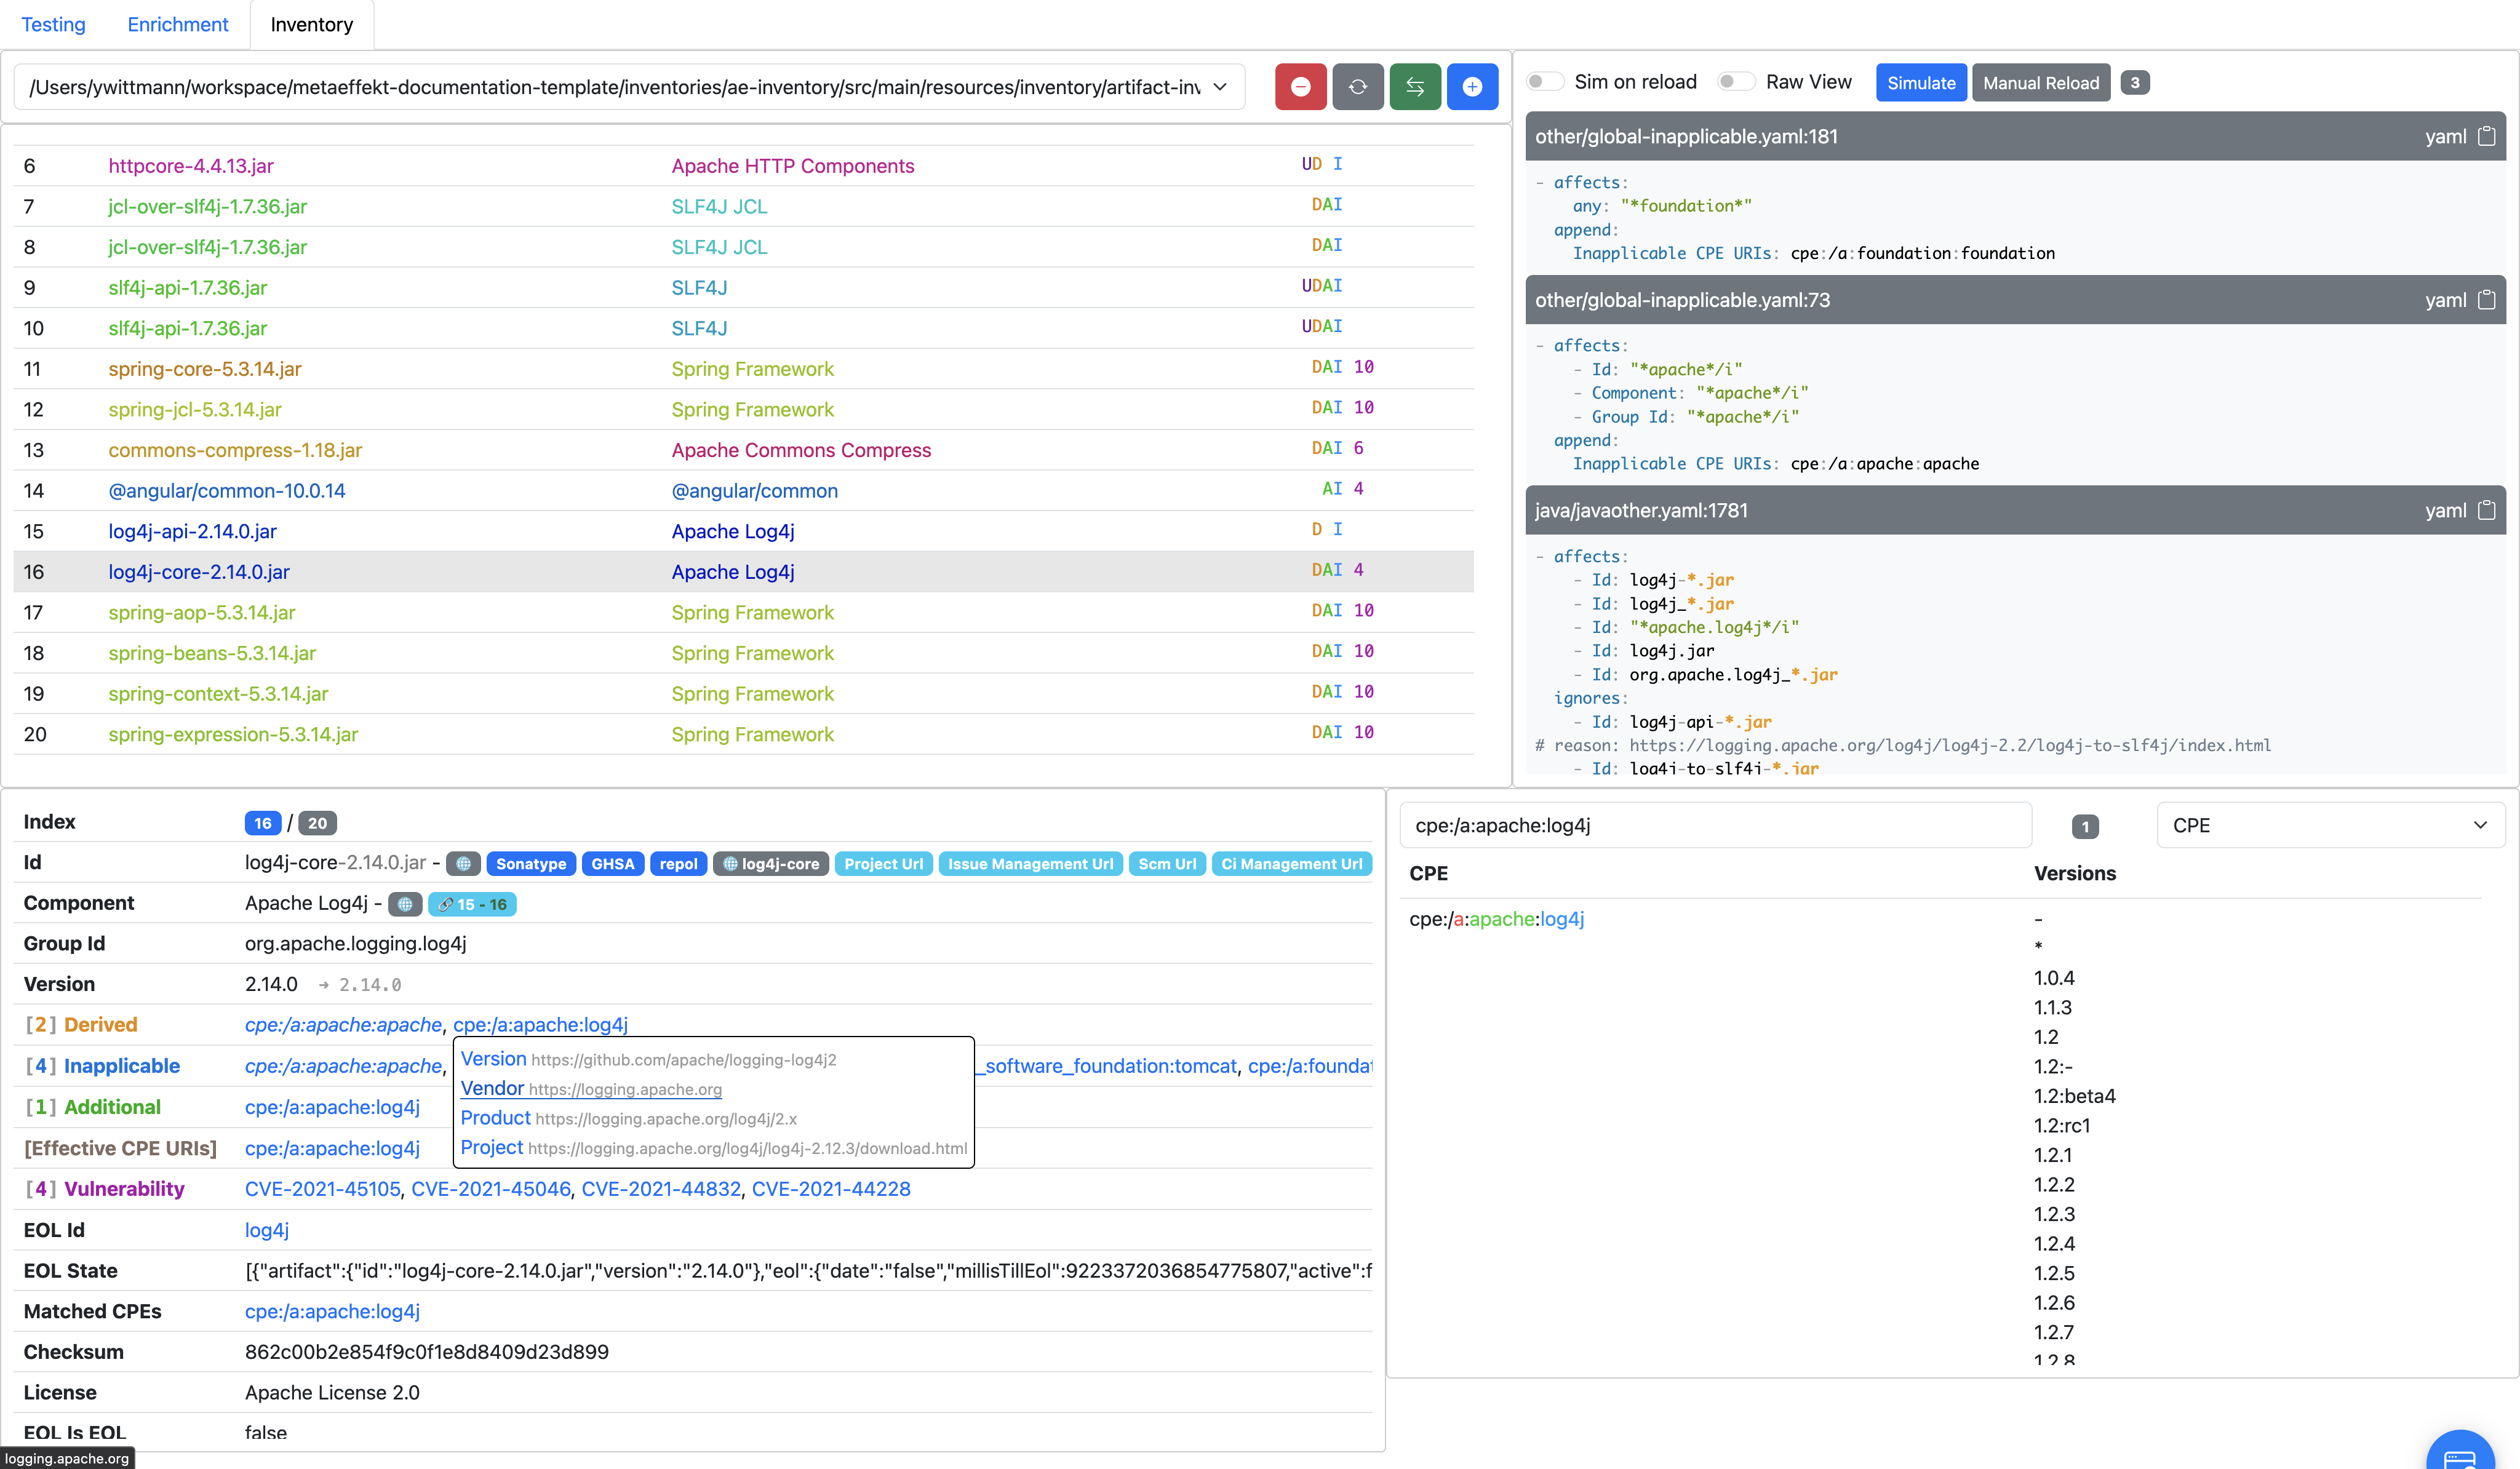
\includegraphics[keepaspectratio,width=1.3\linewidth]{../../images/correlation-utilities-demo}}
    \caption{Das Artefakt \texttt{log4j-core-2.14.0.jar} in den Correlation Utilities}
    \label{fig:correlation-utilities-demo}
\end{figure}

Ein weiteres Widget auf der rechten Seite zeigt, welche Korrelationseinträge auf das aktuelle Artefakt angewendet wurden und erlaubt über eine Integration mit IntelliJ IDEA den direkten Zugriff auf die Korrelationseinträge im Editor und schlägt auf der Basis von einigen bekannten Mustern neue Einträge vor, die mit einem Klick übernommen werden können.
Die Korrelationseinträge werden automatisch bei Änderungen in den Dateien neu geladen und ausgewertet.
Unten rechts kann eine integrierte Abfrageschnittstelle zu den lokalen Datenbanken gefunden werden, über die Abfragen etwa zu \acrshortpl{cpe}, \acrshortpl{cve} oder Produktversionen getätigt werden können.

% TODO: actually perform test, ask Julian
% \smallskip
% Nach einem internen Test hat sich herausgestellt, dass Mitarbeiter mit den Utilities mehr als 2.5-mal so schnell dieselbe Arbeit in höherer Ergebnisqualität durchführen konnten, wie wenn sie dieses Tool nicht verwendet hätten.

\paragraph{Fallunterscheidungen je Artefakt}
Für den allgemeinen Arbeitsablauf mit diesem Tool gibt es pro Artefakt mehrere Fälle, die auftreten können:

\begin{itemize}
    \item Wenn das Artefakt \enquote{Derived CPE URIs} hat, die nicht von einem der weiteren \acrshort{cpe}-Attribute (Additional, Ignores, \ldots) abgedeckt sind, dann bedeutet dies, dass die \acrshortpl{cpe} noch nicht manuell behandelt und geprüft wurden.
    Diese Art von \acrshort{cpe} auf einem Artefakt nennt sich im Tool \enquote{Untouched CPEs}.
    Nachdem sie auf ihre Richtigkeit geprüft wurden, muss die Entscheidung über einen vorhandenen oder neuen Korrelationseintrag in einem der manuellen \acrshort{cpe}-Attribute festgehalten werden.
    Doch nicht nur die automatisch hinzugefügten \acrshort{cpe} müssen untersucht werden, es muss auch nach zusätzlichen \acrshortpl{cpe} im Internet oder den lokalen Datenbanken gesucht werden, um sicherzustellen, dass alle korrekten \acrshort{cpe} gefunden werden.

    \item Wenn das Artefakt nur manuelle \acrshort{cpe}-Attribute gesetzt hat, dann handelt es sich bei diesem Artefakt um ein bereits bekanntes, welches in der Vergangenheit einmal bearbeitet wurde.
    In den meisten Fällen ist hier keine neue Arbeit nötig.
    Manchmal jedoch gibt es Fälle, in denen ein Artefakt seit der letzten Analyse eine neue \acrshort{cpe} zugewiesen bekommen hat, etwas bei dem vorherigen Durchgang übersehen wurde, oder es sich um eine Fehlidentifikation in den Korrelationsdaten handelt und diese fehlerhaft hinzugefügt wurde.
    Je nach Attribut-Kombination sind unterschiedliche Fälle wahrscheinlicher, für welche eine Person mit der Zeit ein Gefühl bekommt.

    \item Wenn das Artefakt überhaupt keine \acrshort{cpe}-Information hat, dann muss manuell nachgeprüft werden, ob es zusätzliche gibt, die diesem Produkt entsprechen.
    Wenn eine oder mehrere passende gefunden werden, wird mit diesen ein neuer Korrelationseintrag angelegt.
\end{itemize}

Vor allem bei einem ersten Durchlauf eines Software-Inventars treten die ersten beiden Fälle häufig auf, aber auch bei erneuten Analysen bekannter Inventare müssen die Artefakte auf ihre Richtigkeit geprüft werden.


\section{Schwächen und Herausforderungen des aktuellen Korrelationsformats}\label{sec:current-correlation-weaknesses}

% https://metaeffekt.atlassian.net/wiki/spaces/KM/pages/3037888514/TBD+New+Correlation+System

Das aktuelle Korrelationsformat hat die letzten Jahre genügend gut funktioniert, um weiterhin verwendbar zu bleiben.
Trotz der hohen Anzahl von über 6400 Korrelationseinträgen von denen die meisten reguläre Ausdrücke auf mehreren Artefaktfeldern prüfen können auch große Software-Inventare in wenigen Sekunden durch alle Einträge geprüft werden (300 Artefakte durchgearbeitet in 3 Sekunden, inklusive Auslesen der Dateien aus dem Dateisystem und Parsen der Einträge).

\subsection{C-01: Übergeneralisierung in Artefakt-Selektoren}\label{subsec:c-01-unspezifische-identifikation-von-artefakten}

% Currently, there are many entries (almost all) that rely on the * wildcard in the Id field to match components version-agnostically. This is not a maintainable approach, since shorter or more common identifiers tend to either be overloaded with multiple components sharing a name, or beginning with the other’s full name. For example:
% - affects:
%     - Id: auth-*.jar
%
% would not only affect an artifact auth-1.2.3.jar, but also auth-registration-helpers-1.2.3.jar. To currently mitigate this, an ignores entry has to be added to the original entry for every single one of these cases.
% - affects:
%     - Id: auth-*.jar
%   ignores:
%     - Id: auth-registration-helpers-*.jar
%
% Fields like the Component cannot be used reliably, since they are often hand-filled or not standardized. Fields like the PURL are more common these days, but still not available on every generated inventory. The artifact Type is still not a normalized field, although it hopefully soon will be (

Wie in \autoref{sec:metaeffekt-inventory-format} erwähnt ist die \texttt{Id} eines Artefakts das einzige Attribut, welches zuverlässig unabhängig des Software-Ökosystems immer gesetzt ist.
Daher dient es in den meisten Korrelationseinträgen auch als Hauptmerkmal, anhand von dem ein Artefakt identifiziert wird.
Leider ist die \texttt{Id} nicht besonders Matching-Freundlich, da sie Versionen und Dateiendungen enthält, sodass bei einem Vergleich nicht auf Gleichheit geprüft werden kann.

Die meisten existierenden Einträge verlassen sich daher auf den Platzhalter (\texttt{*}) im Feld \texttt{Id}, um versionierungsunabhängig zu matchen.
Dieser Ansatz ist aber nicht nachhaltig, da kürzere oder häufig vorkommende Bezeichner von Artefakten zu Mehrdeutigkeiten führen:
So würde ein Eintrag für \texttt{auth-*.jar} sowohl \texttt{auth-1.2.3.jar} als auch \texttt{auth-registration-helpers-1.2.3.jar} erfassen, zur Abhilfe müssen manuell \texttt{ignores}-Einträge für jede Ausnahme erstellt werden.
Felder wie \texttt{Component} mit ihren konkreten Komponentenbezeichnern sind bedauerlicherweise ebenfalls unzuverlässig, da sie teils manuell gepflegt und teils automatisch abgeleitet werden und über Inventare nicht immer einheitlich sind.
Obwohl \acrshort{purl}-basierte Identifikation in den \metaeffekt-Inventaren zunimmt, ist sie bei weitem noch nicht flächendeckend genug verfügbar um diese als Hauptkriterium verwenden zu können.

\subsection{C-02: Inkonsistente und fehlende Artefakt-Typisierung}\label{subsec:c-02-uneindeutige-artefakt-typinformation}

% AE-556: [Artifact Analysis] Define [Artifact Type] / [Component Source Type], create Data Types and apply consistently across code baseTo Do).
% It would be nice if there was a smarter preprocessing step, that would attempt to recover this kind of information in a normalized way, based on several different criteria. The ones listed below are merely examples to illustrate what could be done, this is to be defined:
%     Actual component name
%         Check if there is a PURL and whether it matches with either Component or the Id
%         Check whether the Id contains the Component
%         Fallback to Id
%     Actual component type / ecosystem
%         Consists of a component category (web-module) and a subcategory (nodejs-module)
%         This will be available more generally in the future, but for now this information would have to be guessed from the available fields Type, PURL, etc.
%         This information would be very useful to limit the matching of an entry to a single ecosystem, without affecting others.
%     Version
%         The version field is already fairly normalized, but maybe add a nicer way to compare versions with the component version instead of the huge entry that is currently required for this
% These computed values can be used in the component identification as listed below to reduce the ambiguity in matching and reduce the complexity of the data.
%
% Basically: Enable better, ecosystem-specific matching of artifacts.
% Simply to get the idea across, something like this:
% - affects:
%   - matcher type: maven
%     group id: com.x
%     artifact id: some-artifact

In \autoref{subsec:analysis-ae-software-inventories} wurden die drei Inventar-Attribute \texttt{Type}, \texttt{Specific Type} und \texttt{Ecosystem} identifiziert, auf denen der Typ eines Artefakts \textit{meist} basiert.
Jedoch haben diese mehrere Probleme:

\begin{itemize}
    \item Typbezeichnungen sind auch innerhalb Ökosystemen in manchen Fällen inkonsistent zu sich selbst, indem die Attribute für dasselbe Ökosystem unterschiedliche Wertekombinationen verwenden.
    So sind etwa \texttt{web-module → npm-module}, \texttt{nodejs-module → npm-module} und \texttt{npm-module → <empty>} alle gültige Darstellungsformen für den Typ eines NPM-Moduls.
    Dies verhindert eine normalisierte Klassifikation und erklärt die Notwendigkeit für Ausdrücke wie \texttt{Type: /(web|nodejs|npm)-module/} in der Abfragelogik in den Korrelationseinträgen um alle Ausprägungen mit einem Eintrag abdecken zu können.

    \item Je nach Erzeugungsquelle und den konkreten Ursprüngen der Inventare haben Artefakte nicht immer Typ-Informationen angeheftet.
    So kann man sich nicht immer darauf verlassen, dass ein Typ vorhanden ist und muss auf andere, implizitere Eigenschaften wie Dateiendungen (\texttt{.jar} bei Java-Artefakten) prüfen.

    \item Viele Software-Ökosysteme und Typen haben in den \metaeffekt-Systemen keinen offiziellen Typ, auf den geprüft werden kann oder der gesetzt sein könnte.
    Hierzu zählen etwa Ruby Gems \footnote{\url{https://rubygems.org}} oder Rust mit Crate\footnote{\url{https://crates.io}}, aber auch viele weitere die nicht eindeutig identifiziert werden können.
\end{itemize}

Eine Normalisierung dieser Felder ist seit einiger Zeit geplant, jedoch ist hierzu noch keine Arbeit geschehen.

\subsection{C-03: Duplizierte Artefakt-Selektoren}\label{subsec:c-03-duplizierte-artefakt-selektoren}

% doppelt weil aufeinander aufbauende einträge
% wenn ein feld unterschiedlich gleich neuer eintrag
%   vererbung als lösung

Häufig müssen ähnliche Artefakt-Selektoren für unterschiedliche Korrelationseinträge dupliziert werden.
Aktuell existiert kein Mechanismus zur Vererbung oder Wiederverwendung von Attributen zwischen Korrelationseinträgen.
Wenn sich also eine Produktidentifikation in nur einem Attribut unterscheidet, müssen zwei getrennte Einträge mit fast komplett identischen Attributmengen erstellt werden.
Die einzelnen Attribute, die als Determinate für die übrigen Attributwerte dienen, können leicht variieren und führen so zu redundanten Einträgen mit hohem Wartungsaufwand.

Wie im Beispiel in \autoref{lst:duplicate-artifact-selectors} zu sehen ist, unterscheidet sich die Attributmenge nur in einem Attribut, der \texttt{Architecture}.
Dennoch müssen alleine für diese zwei \enquote{MS Product IDs} zwei nahezu identische Korrelationseinträge gepflegt werden, und in der Realität gibt es wesentlich mehr, die hier angegeben werden müssen.

\begin{lstlisting}[style=yaml,caption={Zwei Korrelationseinträge mit nahezu identischen Attributen},label={lst:duplicate-artifact-selectors}]
- affects:
    - Id: Microsoft Windows 10
      Version: 10.0.19044
      Type: operating system
      Architecture: "64"
    - Id: Windows 10  # no "Microsoft"
      Version: 10.0.19044
      Type: operating system
      Architecture: "64"
  append:
    MS Product ID: "11931"

- affects:
    - Id: Microsoft Windows 10
      Version: 10.0.19044
      Type: operating system
      Architecture: "32"
  append:
    MS Product ID: "11929"
\end{lstlisting}

Dieses Beispiel offenbart ein weiteres Problem der Artefakt-Matcher:
Pro Attribut ist nur ein Wertvergleich möglich.
Sobald es also zwei oder mehr Varianten für ein Feld existieren, müssen entweder reguläre Ausdrücke verwendet, oder der gesamte Eintrag dupliziert werden.

\subsection{C-04: Große Korrelationsdateien als Wartungsproblem}\label{subsec:c-04-groe-und-unubersichtliche-yaml-dateien}

% Find a way to better split the entries into multiple files. The 6000-lines files are not only tedious to work with, but also require unnecessarily large amounts of computational power to render, with a notable slowdown of the IDE in use.
% Maybe, as suggested below, YAML files could not even be required for this, maybe another data format would be better suited. We will see.

Der aktuelle Korrelationsdatensatz der \metaeffektsp umfasst fast 30000 Zeilen an \acrshort{yaml}, die manuell erstellt wurden.
Die Performanz ist wie bereits festgestellt kein Problem, eher die Übersichtlichkeit über diese großen Datenmengen.

\subsection{C-05: Unstrukturierte und unklare Entscheidungsbegründungen}\label{subsec:c-05-reason-not-good-enough}

% The current “reason” format is a simple, unstructured text comment. It is not machine-readable or evaluate-able in any way.
% The current format has a loosely defined arrow reasoning chain syntax that looks like this (fake values) cpe:/a:apache:commons_io --> https://github.com/apache/commons-io --> "library for doing IO operations" --> same library as artifact
% Since the content is only a simple text comment in a YAML file, it is impossible for the parser to extract this information and use it somehow to generate more descriptive views on the reason a connection between components and product identifiers has been made.
% This new format should therefore be in a machine-readable format inside the data structure of the connections. This makes it harder for a human correlation assistant to create the data, therefore the user should not have to edit this reason manually, but rather via a UI that they can click “apply” on or similar.

Wann auch immer ein neuer Eintrag erstellt, eine neue Identifikation hinzugefügt, oder allgemein eine Entscheidung gefällt wird, sollen die entsprechenden Teammitglieder eine textuelle Begründung verfassen, anhand der sich diese später nachvollziehen lassen kann.
Es wurde zudem ein Konsens geschlossen, dass eine schrittbasierte-Syntax verwendet wird, die jeden Schritt in der Herleitungskette einer Information mit einem \enquote{\texttt{-->}} trennt.
Die aktuelle \enquote{reason}-Dokumentation besteht allerdings nur aus einem unstrukturierten Textkommentar über dem Korrelationseintrag im \acrshort{yaml}.
Diese sind nicht maschinenlesbar, oft unvollständig oder vage und werden manchmal aus diversen Gründen nicht angelegt, was die spätere Nachvollziehbarkeit nicht fördert.

Beispielketten können sein:

\begin{itemize}
    \itemsep0em
    \item \texttt{cpe:/a:apache:commons\_io --> https://github.com/apache/commons-io --> "library for IO operations" --> same as artifact}
    \item \texttt{cpe:/a:golang:crypto --> https://github.com/golang/crypto / https://golang.org/x/crypto --> by golang (Go, [mirror] Go supplementary cryptography libraries) --> version range matches artifact}
    \item \texttt{cpe:/a:setorinformatica:sil --> CVE-2024-22633 --> https://tomiodarim.io/posts/cve-2024-22632-3 --> "Setor Informatica is a Brazilian company that develops software for the Brazilian market" / "Smart System for Laboratories (S.I.L.)" --> they reported a vulnerability for another S.I.L. software --> cpe is applicable}
\end{itemize}

\subsection{C-06: Keine Einträge für Negatividentifikationen}\label{subsec:c-06-falle-ohne-aktion-konnen-nicht-dokumentiert-werden}

% If an artifact lacks any CPE or other identifiers, a correlation assistant may have already put in significant effort to reach this point. He might have had to make quite the research or other logical conclusions.
% But, in the current system, such cases \textit{cannot} at all be put into the correlation files. A separate (non-normalized or used) file would have to be used to keep this knowledge. But such an additional system does not exist yet, so nothing is done to document the effort and the information is lost.
% The next time a person sees this artifact and either does not remember the effort from last time, or is a completely new person with a fresh perspective, they cannot build on the research that was already made.

Wenn eine Person ein Artefakt ohne \acrshort{cpe} darauf analysiert, ob diese Abwesenheit korrekt ist, oder ob noch Angaben fehlen und es sich herausstellt, dass das Artefakt tatsächlich keiner \acrshort{cpe} zuordenbar ist, kann der Forschungsaufwand hierfür im aktuellen System nicht dokumentiert werden.
Das liegt daran, dass ein Korrelationseintrag nur dann gültig ist, wenn er eine Selektion und eine Modifikations-Aktion definiert, und damit gibt es keinen Eintrag, auf den die Erkenntnisse notiert werden könnten.
Diese Wissenslücke führt zu wiederholtem Aufwand bei erneuten Analysen desselben Artefakts, da das Wissen über die korrekte Abwesenheit verloren gegangen ist.

\subsection{C-07: Schlechtes Testframework, wenig Unterstützung für automatisierte Kontrolle}\label{subsec:c-07-test-framework}

% The current correlation system does have a “validation” format that allows for the manual creation of test cases for the created correlation entries, but it’s quite tedious to use.
% It would be much nicer, if the system used to create the correlation data (e.g. correlation utilities) would automatically (or with the press of a button) record the artifact the correlation was created on, the before and after states and create a test case with an expected result based on that.
% Through the more documentation-heavy new format, these tests may also already be self-documenting.

Existierende Testfälle für Korrelationseinträge werden manuell in einem separaten Validierungsformat gepflegt, was in seiner Konfiguration aufwendig ist.
Dieser Aufwand führt dazu, dass es in der Realität nicht von den Mitarbeitern verwendet wird, und so nur ein sehr kleiner Datensatz an automatisierbaren Testfällen existiert.

\subsection{C-08: Generierte YAML-Dateien}\label{subsec:c-08-generated-correlation-data}

% The generated directory contains several automatically generated YAML correlation files, based on the data that is present in the index when generating.
% These need to be converted into the new format somehow.

Die automatisch generierten \acrshort{yaml}-Dateien, wie in \autoref{subsec:old-generated-correlation-data} gezeigt, müssen bei Datenänderungen manuell neu generiert werden, was nicht intransparent ist.
Zudem haben sich, vor allem bei den JRE/JDK-Generatoren einige Probleme mit der Abbildung auf das aktuelle Korrelationssystem gezeigt, die nur über die Verwendung von inkrementellen Korrelationseinträgen und dem Attribut \texttt{CPE URIs} (welches nicht mehr verwendet werden soll) gelöst werden konnten.
Da eine der Anforderungen an das neue Korrelationssystem ist, weitere dynamische Quellen zu integrieren, muss dieses Konzept für generierte Daten von Anfang an mitgedacht werden.

\subsection{C-09: Teilen öffentlicher Anteile}\label{subsec:c-09-sharing-of-public-data}

% darüber reden, dass der terms metadata-datensatz ja auch mit dem Kosmos https://github.com/org-metaeffekt/metaeffekt-kosmos die öffentlichen aspekte freigibt
% man könnte das hier ja genau so machen, aber im moment ist alles ein gemischter datensatz
% im neuen inkrementellen konzept soll das am besten über mehrere datenquellen auftrennbar sein
% daten die aus öffentlichen datenquellen abgeleitet wurden

Der aktuelle Korrelationsdatensatz besteht im Moment zu einem Teil aus den generierten Korrelationseinträgen aus öffentlichen Datenquellen, und zum anderen aus unternehmensintern für spezifische Kunden recherchierten Daten.
Da diese Daten direkt nebeneinander in den gleichen Verzeichnissen liegen, erschwert dies die Auftrennung.
Da in dem manuellen Teil dieses Datensatzes viel Firmenzeit geflossen ist, stellt dieser einen der lizenzierbaren Bausteine der \metaeffektsp dar und ist damit nur kostenpflichtig erwerblich.

Analog zum bereits existierenden \enquote{\metaeffekt-kosmos}-Projekt\footnote{\url{https://github.com/org-metaeffekt/metaeffekt-kosmos}}, welches den Open-Source-Anteil der \metaeffekt-Lizenzdatenbank öffentlich frei verfügbar zugänglich macht, könnte ein Konzept eingeführt werden, bei dem die automatisch generierten Einträge ohne die manuellen Arbeiten auf eine ähnliche Weise verfügbar gemacht werden, damit jeder eine gewisse Grundqualität der Ergebnisse erhält.
So können firmeninterne Ergänzungen weiterhin in einem separaten, nicht öffentlichen Datensatz verteilt werden.

\subsection{C-10: Reihenfolgenbedingte Seiteneffekte von Einträgen}\label{subsec:c-10-order-dependency}

% Die inkrementelle Anwendung von Korrelationseinträgen erfordert eine strenge Reihenfolge, die aktuell nur durch die Position in der \acrshort{yaml}-Datei gesteuert wird. Änderungen in der Eintragsreihenfolge können unbeabsichtigte Seiteneffekte verursachen. Explizite Abhängigkeitsdeklarationen oder eine deklarative Priorisierungslogik (anstatt impliziter Dateiordnung) würden Robustheit und Verständlichkeit erhöhen.

Das aktuelle System für Korrelationseinträge verarbeitet die Daten inkrementell (siehe \autoref{par:incremental-correlation-entries}), d.h.\ jeder Eintrag baut potenziell auf dem Zustand auf, der durch vorherige Einträge erarbeitet wurde.
Da diese Abhängigkeiten zwischen Einträgen nicht explizit deklariert werden müssen, ergibt sich die Reihenfolge innerhalb einer \acrshort{yaml}-Datei wenigstens noch basierend auf der Position innerhalb der Datei, Dateiübergreifend jedoch ist die Verarbeitungsreihenfolge arbiträr basierend auf der Ordnung, die das Dateisystem dem Programm übergibt.
Dies macht das System empfindlich gegenüber Umordnungen der Einträge, vor allem wenn über Dateien hinweg absichtlich oder unabsichtlich Abhängigkeiten erstellt wurden.

Ein Beispiel für eine solche Situation ist in \autoref{lst:correlation-order-depdendency-example} dargestellt, deren beide Korrelationseinträge in zwei separaten Dateien aufgeführt sind.
Der erste Eintrag ergänzt eine Liste an \acrshortpl{cpe} ganz allgemein für \texttt{redis}-Artefakte in dem \texttt{Additional CPE URIs}-Attribut.
Der zweite hat nun das Ziel, diese für das Python-Modul \enquote{redis}\footnote{\url{https://pypi.org/project/redis}} als nicht zutreffend zu markieren.
Dafür müssen die \acrshort{cpe} über das \texttt{remove}-Schlüsselwort zunächst wieder aus dem \texttt{Additional CPE URIs}-Attribut entfernt, und dann explizit als \texttt{Inapplicable CPE URIs} für das Python-Modul gesetzt werden.
Wenn nun die Verarbeitungsreihenfolge der Einträge sich durch eine Verschiebung oder Umbenennung der Dateien ändert, dann wird auch diese Logik nicht mehr korrekt greifen können.

\begin{lstlisting}[style=yaml,caption={Korrelationseinträge in zwei unterschiedlichen Dateien, die aufeinander aufbauen},label={lst:correlation-order-depdendency-example}]
- affects:
    - Id: redis-*/i
      Component: redis/i
  append:
    Additional CPE URIs: cpe:/a:redis:redis, cpe:/a:redislabs:redis, cpe:/a:pivotal_software:redis
    EOL Id: redis
- affects:
    - Id: redis-*/i
      Type: python-module
  remove:
    Additional CPE URIs: cpe:/a:redis:redis, cpe:/a:redislabs:redis, cpe:/a:pivotal_software:redis
  append:
    Inapplicable CPE URIs: cpe:/a:redis:redis, cpe:/a:redislabs:redis, cpe:/a:pivotal_software:redis
    Additional CPE URIs: cpe:/a:redis:redis-py
\end{lstlisting}

\subsection{C-11: YAML-Eintrag finden}\label{subsec:c-11-finding-yaml-entries}

Die Correlation Utilities, wie in \autoref{subsec:correlation-utilities} vorgestellt, erlauben es mit einem Klick auf einen Korrelationseintrag zu diesem in der entsprechenden \acrshort{yaml}-Datei zu springen.
Das Problem hierbei liegt darin, dass das aus dem \acrshort{yaml} erzeugten Datenmodell von sich aus keine Referenz mehr auf die Zeilennummern der Datei enthält.
Weiterhin werden einige Transformationen an den Attributen vorgenommen, wie etwa das Parsen der unterschiedlichen Darstellungsweisen für reguläre Ausdrücke, sodass nicht mehr einfach so die Originalinhalte mit dem Datenmodell abgeglichen werden können.
Es wird daher im Quelltext der \acrshort{yaml}-Dateien Zeile für Zeile jeder Eintrag nach gewissen Schlüsselwörtern aus dem Datenmodell abgesucht, und der mit der höchsten Übereinstimmungsrate wird ausgewählt.

Dieser Prozess funktioniert bei einer großen Anzahl der Einträge, jedoch kann es bei sehr ähnlichen Einträgen oder jenen, die viele komplizierte reguläre Ausdrücke verwenden passieren, dass die Zuordnung nicht erfolgreich ausgewertet wird.


\section{Anforderungen an das neue Korrelationssystem}\label{sec:requirements}

% “4.3. Data Types in Falcon” ([Cheramangalath et al., 2016, p. 6](zotero://select/library/items/4DG8G9J3)) ([pdf](zotero://open-pdf/library/items/QNYKYEH4?page=6&annotation=C7MKFAUG))

Basierend auf der Analyse der bestehenden Herausforderungen und weiteren Rahmenbedingungen werden die Anforderungen an das neue Korrelationssystem abgeleitet.

\subsection{A-01: Graphenbasiertes Datenmodell mit expliziten Abhängigkeitsdeklarationen}\label{subsec:req-format-product-graph}

Das Kernmodell des neuen Systems muss als gerichteter Graph implementiert werden, wobei Knoten typisierten Produktrepräsentationen (Artefakte, \acrshort{cpe}, \acrshort{eol}-Id, MS Product ID) repräsentieren und Kanten Relationen mit unterschiedlichen Typen zwischen diesen darstellen.
Kantentypen umfassen mindestens \enquote{is} (represented by, positive Zugehörigkeit) und \enquote{is not} (not represented by, expliziter Ausschluss).
Der Typ des Zielknotens einer Relation entscheidet, wie die Art der Relation interpretiert werden soll.

Jede Repräsentation eines Produkts darf sich in nur einen Knoten ausprägen, Mehrfachreferenzen auf dieselbe Repräsentation müssen durch Kanten auf einen einheitlichen Knoten dargestellt werden.
Dies löst die Reihenfolgenabhängigkeit (\hyperref[subsec:c-10-order-dependency]{C-10}), indem die Abhängigkeiten zwischen Knoten explizit deklariert werden.
Diese Deklaration soll eine topologische Sortierung während der Verarbeitung erzwingen und implizite Dateireihenfolgeabhängigkeiten vollständig entfernen.

Um die programmatische Erfassung eines Knotenpunktes zu ermöglichen, soll jeder Knotenpunkt einen textuellen Identifikator besitzen, der in Kombination mit dem Knotentyp im Graph eindeutig ist.
So kann über die Typ-Id-Kombination jeder Knoten im Graph angesprochen werden.

Der Graph ist gerichtet, damit über die Kantenrichtung die \enquote{is}- und \enquote{is not}-Beziehungen klar ausgewertet werden können.
Falls es nötig ist, kann eine identische, umgekehrte Kante dazu verwendet werden, um die Richtung der Kante auf beide Seiten zu erweitern.
In den Fall, dass der Bedarf besteht herauszufinden, welche weiteren Repräsentationen eine Produktrepräsentation noch haben kann, muss damit also bei dem als \enquote{sich selbst} identifizierten Knoten eine Durchquerung des Graphen unter Berücksichtigung der Kantenrichtung- und Typen gestartet werden, bis alle erreichbaren Knoten gefunden und ausgewertet wurden.

Mit diesem System sollen jedwede Produkte und Repräsentationen modelliert werden können.
Dies löst die Herausforderung \hyperref[subsec:c-06-falle-ohne-aktion-konnen-nicht-dokumentiert-werden]{C-06}, dass keine Identifikationen ohne bekannte Relationen modelliert werden können, da in diesem System dennoch ein Knotenpunkt für die Identifikation erstellt werden kann, ohne eine Relation zu einem weiteren Knoten erstellen zu müssen.

\subsection{A-02: Produkt-Konzept}\label{subsec:req-product-concept}

Wichtig ist die Unterscheidung zwischen einem \textit{Produkt}, und der \textit{Repräsentation eines Produkts} (she.\ \autoref{subsec:produkte-vs-reprasentation}).
Diese sollen sich zwar im Graphen beide als Knotenpunkte darstellen, jedoch muss zwischen ihren Typen unterschieden werden.

So könnte eine Repräsentation mit einer Kante auf einen Produkt-Knotenpunkt verweisen und von diesem eine Kante auf eine weitere Repräsentation des Produkts um anzugeben, dass diese Repräsentationen das selbe Produkt darstellen.

Produktknoten sollen in der Lage sein, Metainformationen über die zugehörigen Repräsentationen abzulegen.
Dazu gehören vor allem Informationen über die Versionsräume und wie zwischen diesen umgewandelt werden kann.

\subsection{A-03: Normalisierte Typidentifikation und typspezifische Attribute für Software-Artefakte}\label{subsec:req-type-specific-matching}

Um die Herausforderung \hyperref[subsec:c-02-uneindeutige-artefakt-typinformation]{C-02} der multiplen Ausprägungen und inkonsistenten Typinformationen zu lösen muss eine Typinferenz-Logik den Artefakttypen konsistent aus multiplen Quellen aufbereiten.
In \autoref{subsec:analysis-ae-software-inventories} wurden die häufigsten Muster für Typinformationen analysiert.
Die Ausgabe der Typinterferenz soll diese verwenden, um normalisierte Ökosystembezeichner (z.B. \texttt{java-module}, \texttt{npm-package}, \texttt{python-module}), als Artefaktattribut verfügbar machen.

Basierend auf dem erkannten Ökosystem/Typ eines Artefakts werden dann weitere Extraktoren auf die Artefakt-Metadaten angewendet.
Diese müssen weitere Attribute als First-Class Matching-Kriterien auf den Artefakt-Selektoren zur Verfügung stellen, wie etwa Maven-Koordinaten (Group Id, Artifact Id) für Java, Paketnamen für NPM, Distributionskennung für Linux-Pakete, Java Runtime-Provider, \ldots.
Wildcard-Selektor wie bisher häufig in der \texttt{Id} (\hyperref[subsec:c-01-unspezifische-identifikation-von-artefakten]{C-01}) können so durch exakte, ökosystemspezifische Attributvergleiche ersetzt werden.

\subsection{A-04: Vererbung von Artefaktmerkmalen}\label{subsec:req-selektor-inheritance}

Um zu vermeiden, dass Artefakt-Selektoren wie in \hyperref[subsec:c-03-duplizierte-artefakt-selektoren]{C-03} für ähnliche Identifikationen wiederholt werden müssen, soll es ein Vererbungssystem an Artefakt-Selektoren geben.
Ein Basis-Selektor definiert generische Selektorattribute (z.B.\ für alle Microsoft Windows-Varianten), während abgeleitete Selektoren spezifische Erweiterungen (z.B.\ Architektur) hinzufügen, wobei lokale Attributdefinitionen geerbte überschreiben.
Dies erlaubt das Teilen von Basisattributen zwischen mehreren spezifischeren Ausprägungen eines Artefakts, ohne die Basisattribute bei jeder Ausprägung wiederholen zu müssen und vermeidet damit zu pflegende Redundanz.
So muss ebenfalls nur der Basis-Selektor angepasst werden, wenn neue Attribute dazukommen oder vorhandene bearbeitet werden sollen.

\subsection{A-05: Auflistung mehrerer Werte pro Attribut}\label{subsec:req-multiple-attribute-values}

In \hyperref[subsec:c-03-duplizierte-artefakt-selektoren]{C-03} wurde die Herausforderungen der mehreren Werte pro Attribut aufgeführt.
Um dieses zu lösen, soll im neuen Modell ein Abgleich von mehreren Optionen möglich sein, bei der nur ein Attributwert übereinstimmen muss (oder-Verknüpfung).

\subsection{A-06: Unterstützung regulärer Ausdrücke}\label{subsec:req-regex-support}

Auch wenn im neuen Format über \hyperref[subsec:req-type-specific-matching]{A-03} die Anzahl der Wildcard-Selektor drastisch verringert werden, soll dennoch das in \autoref{sec:current-correlation-format} beschriebene inkrementelle Wildcard-System weiterhin bestehen bleiben.

\subsection{A-07: Manuelle Modifikation des Graphen}\label{subsec:req-manual-format-modification}

Da in dem neuen Korrelationssystem noch immer manuelle Korrekturen an der automatischen Erkennung von \acrshort{cpe} gemacht werden können sollen, muss ein neues \acrshort{yaml}-basiertes Format entwickelt werden, welches einen solchen Produkt-Graphen modifizieren kann.
Die durchführbaren Modifikationen am Graphen müssen mindestens die Erstellung, Modifikation und Entfernung von Knotenpunkten jedes Types, und die Erstellung, Modifikation und Entfernung von Kanten zwischen Knoten beinhalten.
Technisch sollte dieses Modifikationsformat auf eine Weise modelliert werden, dass jegliche nötigen Modifikationen am Graphen ausschließlich darüber lösbar sind, ohne weiteren Code schreiben zu müssen, um als allgemeine Schnittstelle für Graphmodifikationen zu dienen.
Auf diese Weise können auch andere Prozesse die selbe Logik verwenden, um ihre Änderungen durchzuführen, mit den gleichen Garantien wie der manuelle Prozess.

Da die Kombination aus Typ und Id jedes Knotens im Graphen eindeutig ist (she. \hyperref[subsec:req-format-product-graph]{A-01}), sollte auch das Modifikationsformat diese Weise verwenden, Knotenpunkte für die Modifikation zu selektieren.

Das neue Korrelationssystem als Graph zu modellieren führt viele Komplexitäten ein, die für den Nutzer im manuellen Modifikationsformat abstrahiert werden müssen, um noch immer so effektiv wie im alten Format arbeiten zu können.
Hierfür muss ein Format iterativ entworfen und mit aktuellen Nutzern des Formats getestet und abgesprochen werden, um es so einfach wie möglich zu machen, den Graphen zu modifizieren ohne Kontrolle über detaillierte Attribute zu verlieren.

Da das alte Format oft Schwierigkeiten hatte, aus dem Datenmodell wieder die ursprünglichen Einträge in den \acrshort{yaml}-Dateien zu finden (she.\ \hyperref[subsec:c-11-finding-yaml-entries]{C-11}), soll in dem neuen \acrshort{yaml}-Modifikationsformat das Auffinden von Einträgen deterministisch gestaltet werden.
Wenn zur Selektion der Knotenpunkte im \acrshort{yaml} der Typ und die Id verwendet wird, dann kann diese auch umgekehrt wieder aus dem Graphen ausgelesen und die zugehörige Zeile im \acrshort{yaml} gefunden werden.

\subsection{A-08: Maschinenlesbare Entscheidungsdokumentation}\label{subsec:req-reason-format}

Um Daten wie Projektreferenzen, Beschreibungen und Begründung für Entscheidungen im Gegensatz zum alten Korrelationssystem (\hyperref[subsec:c-05-reason-not-good-enough]{C-05}) maschinenlesbar zu machen, müssen die bisherigen Kommentarfelder als strukturierte Objekte mit standardisierten Feldern modelliert werden.
Dies soll es in automatisierten Systemen oder Nutzeroberflächen möglich machen, Metadaten über die Produktidentifikationen nützlicher anzuzeigen und auswerten zu können.

Da das neue Korrelationssystem mit einem Graphen modelliert wird, gibt es zwei Stellen, an denen diese Dokumentation angebracht werden kann und muss.
So wird der frühere \texttt{\# reason:}-Kommentar mit der Begründung der gegenseitigen Anwendbarkeit von Produkten nun auf den Kanten modelliert, und die weiteren Metadaten eines Produkts wie die Beschreibung oder Web-Referenzen auf den Knotenpuntken.

\subsection{A-09: Generierungsframework für dynamische Daten}\label{subsec:req-generated-data}

Im aktuellen Korrelationssystem liegen die generierten \acrshort{yaml}-Dateien gleichwertig neben den manuell gepflegten Daten (\hyperref[subsec:c-08-generated-correlation-data]{C-08}).
Da ihre Existenz nicht von Beginn an geplant war, wurden das Selektor-System und die weiteren Matching-Regeln nicht für die besonderen Anforderungen die diese Quellen mit sich bringen ausgelegt.
Im neuen System soll der gesamte Graph darauf aufbauen, dass er zunächst mit generierten Daten befüllt wird und basierend darauf die manuellen Modifikationen angewendet werden.

Mit den Datensätzen der \metaeffektsp sollen bereits alle Knotenpunkte für \acrshortpl{cpe}, MS Product Ids und \acrshort{eol}-Ids erzeugt werden, die bekannt sind, manche sollen bereits Kanten zwischen den Knoten erzeugen.
Zudem sollen weitere Datenquellen wie die bereits vorhandenen Generatoren für NPM-Pakete zu \acrshortpl{cpe} und die für die vielen Java Runtimes, aber auch neue wie purl2cpe von scanoss\footnote{\url{https://github.com/scanoss/purl2cpe}} dazu beitragen, den Graphen bereits vorzufüllen und die darauf folgende Arbeit zu erleichtern.

Um den fertigen auslieferbaren Graphen zu erhalten, soll zunächst der generierte Anteil des Graphen erstellt werden und dann auf diesem mit den manuellen Modifikationen aufgebaut werden.
Durch diese Trennung in mehrere \enquote{Contributors} am Graphen kann \hyperref[subsec:c-09-sharing-of-public-data]{C-09} einfach abgebildet werden, indem der Datensatz vor der Anwendung des manuellen Schritts ausgeliefert wird.

\subsection{A-10: Qualitätsmetriken des Graphen}\label{subsec:req-graph-inner-consistency}

%- Innere Konsistenz: Zu jeder Repräsentation, die durch das Modell identifiziert werden soll, darf maximal eine
%  eindeutige Identifikation stattfinden und es darf keine losen Knoten geben
%- Datensatz erklärt sich selbst: Zu jedem Eintrag und jeder Verbindung muss es eine Begründung jeglicher Art geben
%- Ein sich selbst prüfender Datensatz: Nachdem ein Datensatz manuell geprüft wurde, werden alle Identifikationen in
%  einem separaten Datensatz abgelegt, um bei zukünftigen Änderungen automatisch geprüft werden zu können. So soll
%  gegeben sein, dass die Identifikation eines bekannten Produktes nicht einfach so ändern kann, ohne, dass man es
%  mitbekommen würde.

Um verifizieren zu können, dass der Graph sinnhaft strukturiert und in sich selbst konsistent ist, müssen einige Prüfungen darauf ablaufen können.
Diese prüfen mindestens die folgenden Eigenschaften:

\begin{itemize}
    \item Zu jeder Repräsentation eines Produkts in dem Graphen darf maximal genau eine eindeutige Identifikation stattfinden.
    Dies bedeutet, dass jeder Knoten exakt eine Repräsentation vollständig modellieren sollte und diese nicht noch einmal von einem anderen Knoten partiell abgedeckt sein darf.
    Diese Metrik muss sowohl in dem Matching-Algorithmus, als auch als Modellierungsvorschrift umgesetzt werden.
    % FIXME-YWI: das hier hat halt das Problem, dass wir den Graphen mit allen CPE, etc. füllen wollen und nicht immer ein zugehöriges Produkt erzeugt werden kann.
    \item Es darf keine losen Knoten geben, jede Repräsentation muss mindestens zu einem Produkt-Knotenpunkt verbunden sein um sicherzustellen, dass mit einer Identifikation auch ein Informationsgewinn stattfinden kann.
    \item Um einen sich selbst erklärenden Datensatz zu erhalten, müssen die Metadaten jedes Knotenpunktes aufgefüllt sein und die Kanten eine Begründung enthalten, warum sie so existieren.
    \item Der Graph soll sich selbst prüfen können: Nachdem ein Software-Inventar manuell geprüft wurde, sollen alle Quell-Artefakte mit ihren Identifikationen in einem separaten Datensatz abgelegt werden, um diese bei zukünftigen Änderungen am Graphen automatisch prüfen zu können.
    So kann die Identifikation eines bekannten Produktes sich nicht einfach so ändern, ohne, dass man es mitbekommen würde.
    \item Eine Prüfung auf zirkuläre Vererbungs-Referenzen soll sicherstellen, dass es immer einen spezifischeren Knoten gibt und keine Schleife entsteht.
\end{itemize}

\subsection{A-11: Organisation der \acrshort{yaml}-Dateien}\label{subsec:req-yaml-file-organization}

Die manuell gepflegten Korrelationsdateien werden noch immer im Dateisystem abgelegt werden.
Hierbei müssen jedoch die Herausforderungen der tausenden Zeilen langen \acrshort{yaml}-Dateien adressiert werden (\hyperref[subsec:c-04-groe-und-unubersichtliche-yaml-dateien]{C-04}).
Es soll für die neuen Dateien mindestens eine Auftrennung in Verzeichnissen nach Typ und/oder Ökosystem geben, und weiterführend können die einzelnen Hersteller- oder Produktgruppen jeweils in getrennten Dateien aufgeführt werden.

\subsection{A-12: Überführung von Einträgen aus dem alten Korrelationsdatensatz}\label{subsec:req-current-dataset-conversion}

Um die Transition zum neuen Korrelationssystem so einfach wie möglich zu machen, sollen die beiden Datensätze zunächst parallel weiter geführt und auf Inventare angewendet werden.
In der Transitionsperiode sollen dann die Einträge aus dem alten Format in das neue konvertiert und damit der alte langsam ersetzt werden.

Dazu muss sichergestellt werden, dass der neue Graph mindestens die Fähigkeiten des alten Formats abdeckt und durch seine weiteren Eigenschaften die Identifikation sogar verbessert.

\subsection{A-13: Performance des neuen Korrelationsformats}\label{subsec:req-correlation-format-performance}

Das alte Korrelationssystem wurde bei unterschiedlichen Inventar-Größen mit dem aktuellen Datensatz mit 6400 Einträgen getestet.
Die Zeiten werden in \autoref{tab:old-correlation-performance} angegeben.

Aus diesen Messwerten sind zwei Phasen erkennbar.
Zunächst läuft eine konstante Startzeit (bei dem getesteten Datensatz etwa 0,8-0,9 Sekunden), die unabhängig von der Anzahl der Artefakte im Inventar auftritt, in welcher die Korrelationseinträge aus dem \acrshort{yaml} ausgelesen werden.
Danach steigt die Laufzeit annähernd linear mit der Anzahl der Artefakte an, der Zeitbedarf pro zusätzlichem Artefakt ist also relativ konstant.

\begin{table}[h!]
    \centering
    \label{tab:old-correlation-performance}
    \begin{tabular}{l r r r r}
        \toprule
        \textbf{Artefakte} & \textbf{Ø [s]} & \textbf{Min. [s]} & \textbf{Max. [s]} \\
        \midrule
        0                  & 0,806          & 0,435             & 1,668             \\
        1                  & 0,897          & 0,453             & 1,919             \\
        500                & 2,033          & 1,504             & 3,277             \\
        1000               & 3,256          & 2,531             & 4,612             \\
        2000               & 5,920          & 4,543             & 6,979             \\
        3000               & 8,804          & 7,425             & 11,800            \\
        4000               & 9,433          & 8,780             & 10,338            \\
        5000               & 12,162         & 10,929            & 13,596            \\
        6000               & 13,609         & 12,461            & 15,381            \\
        \bottomrule
    \end{tabular}
    \caption{Gemessene Laufzeiten des alten Korrelationsformats bei unterschiedlichen Artefakt-Anzahlen.}
\end{table}

Da der Korrelationsschritt bisher bei weitem nicht der zeitintensivste Schritt in der Schwachstellenanalyse ist, ist die Optimierung nie eine kritische Anforderung gewesen.
Das neue Korrelationsmodell sollte diese Zeiten jedoch bei vergleichbaren Datenmengen dennoch nicht um einen Faktor von 2 überschreiten.

% \begin{table}[h!]
%     \centering
%     \label{tab:new-correlation-performance}
%     \begin{tabular}{l r r r}
%         \toprule
%         \textbf{Artefakte} & \textbf{Ø [s]} & \textbf{Min. [s]} & \textbf{Max. [s]} \\
%         \midrule
%         0                  & 0,000          & 0,000             & 0,000             \\
%         1                  & 0,034          & 0,001             & 0,134             \\
%         500                & 2,303          & 2,078             & 2,950             \\
%         1000               & 4,249          & 4,022             & 4,790             \\
%         2000               & 8,582          & 8,109             & 9,658             \\
%         3000               & 12,639         & 12,156            & 13,730            \\
%         4000               & 16,702         & 16,113            & 17,446            \\
%         5000               & 20,693         & 20,179            & 21,175            \\
%         6000               & 24,601         & 24,093            & 25,503            \\
%         \bottomrule
%     \end{tabular}
%     \caption{Laufzeiten des neuen Korrelationsformats bei unterschiedlichen Artefakt-Anzahlen.}
% \end{table}

\subsection{A-14: Auslieferung des Datensatzes}\label{subsec:req-correlation-data-delivery}

Der Aufwand, den Korrelationsdatensatz zu verteilen, muss vergleichbar mit dem alten Korrelationssystem sein.
Bisher hat es ausgereicht, einen Ordner an \acrshort{yaml}-Dateien zu verteilen.
Es darf also keine dedizierte Ausführungsumgebung einer Datenbank vorausgesetzt werden, der gesamte Ablauf muss innerhalb des Java-Prozesses stattfinden, in dem auch das alte Format verwendet wird.


\section{Referenzfälle}\label{sec:reference-case-chapter}

Aus einer Auswertung aus dem bereits vorhandenen Korrelationsdatensatz wurden vier grundlegende Fälle identifiziert, die in ihrer Kombination den Großteil der Komplexität in den bisherigen Daten abdecken.
Sie wurden nicht aufgrund von ihren Inhalten oder betreffenden Produkten gewählt, sondern wegen ihrer Struktur und verwendeten impliziten oder expliziten Mechanismen.
Das neue Modell muss also mindestens diese Fälle abdecken können und daher werden sie als Referenzfälle verwendet.

Neben dem konzeptionellen Unterschied zum neuen Korrelationsformat der Modellierung als Graphen haben diese Beispiele im alten Format zudem die Eigenschaft, dass sie mit dem Ziel erstellt werden, ein Inventar-Artefakt zu modifizieren.
Es wird also immer ausschließlich von einem Artefakt ausgegangen, und dessen Ziel-Attribut-Werte definiert.
Im neuen Format wird dieser Gedanke in den Hintergrund treten, und sich implizit durch den Aufbau des Graphen ergeben.

Es werden zunächst immer die Einträge vorgestellt, dann die Herausforderungen und relevanten Anforderungen identifiziert.
Diese Referenzfälle werden in \autoref{sec:beispiele-fertige-implementierung} jeweils auf das neue Korrelationssystem übersetzt, um einen Vergleich der Formate zu ermöglichen.

% FIXME-KKL: Zusammenhalten: Ich glaube der Kommentar hier bezieht sich darauf, dass im PDF zwischen dem Titel und der Klammer ein Abstand ist. Den habe ich schon versucht wegzubekommen, aber LaTex will das unbedingt so aufteilen.
\paragraph{JavaScript-Paket mit multiplen Namensvarianten}\label{par:reference-case-walletconnect} (s. \autoref{lst:correlation-generated-walletconnect-example})

Bei dem Paket \texttt{@web3-react/walletconnect} handelt sich in der NPM-Registry zwar um ein eindeutiges Paket, allerdings kann sich der Bezeichner in den gescannten Software-Inventaren in unterschiedlichen Varianten ausprägen, auf die alle geprüft werden muss.
In diesem Fall handelt es sich um eine Positividentifikation auf einer \acrshort{cpe} \texttt{cpe:/a:uniswap:web3-react\_walletconnect}, die als \texttt{Additional CPE URIs} zum Artefakt hinzugefügt wird.
Um die drei alternative Namensformen in dem Selektor in der \texttt{affects}-Sektion erfassen zu können, müssen diese alle separat mit Wiederholung der restlichen Attribute in alternativen Selektoren geführt werden.
Über dem Eintrag ist ein \texttt{reason}-Kommentar, der eine Referenz auf das Paket auf NPM und auf die Homepage des Herstellers enthält.

Dieser Fall, wie auch die folgenden, demonstriert die Notwendigkeit, ökosystemspezifisch-normalisierte Bezeichner zu extrahieren (\hyperref[subsec:req-type-specific-matching]{A-03}).
Die \enquote{-*}-Suffixe können zu einer Übergeneralisierung der Einträge führen, aber auch der häufig wiederholte reguläre Ausdruck \texttt{/(web|nodejs|npm)-module/} für die Erkennung des Artefakt-Typen kann zu Fehlern führen und stellt die üblichen Probleme von Redundanz dar.

\hyperref[subsec:req-multiple-attribute-values]{A-05} ist aus der Notwendigkeit entstanden, innerhalb eines Eintrages die Wiederholung nah identischer Selektoren zu vermeiden.
In diesem Fall war es nötig, für jede Namensform einen neuen Selektor zu erstellen, und alle weiteren Attribute zu wiederholen.

\paragraph{Java-Runtimes: Komplexe Versionstransformation}\label{par:reference-case-java-runtimes} (s. \autoref{lst:reference-case-java-runtimes})

Wie in \autoref{subsec:old-generated-correlation-data} bereits gezeigt, wird ein wesentlicher Teil des alten Korrelationsdatensatzes regelmäßig automatisch in einem dedizierten Prozess generiert.
Das Listing zeigt einen Auszug der generierten Einträge für die Java-Runtime \enquote{Amazon Corretto} und \enquote{Azul Zulu}.
Diese wurden einmal aus der Notwendigkeit eingeführt, da die \acrshortpl{cpe} der Java Runtimes einige der wenigen sind, bei denen häufig der Update-Part tatsächlich verwendet wird und andererseits die Versionen der \acrshortpl{cpe} selbst innerhalb eines Vendor-Product-Namensraums sehr uneinheitlich strukturiert sein können.
Einige häufige Beispiele für das Format der Version- und Update Parts sind: \texttt{21.0.6:*}, \texttt{23:*}, \texttt{*:update32}, \texttt{*:update\_32}, \texttt{1.6.0:update32\_b31}, \texttt{1.6.0:update32\_b32}.
Für jede dieser Versionen ist ein neuer Eintrag in den \acrshort{yaml}-Dateien nötig, da jeder Eintrag nur eine versionierte \acrshort{cpe} adressieren kann.

Die zugehörige Anforderung für die automatische Befüllung des Graphen ist \hyperref[subsec:req-generated-data]{A-09}.
Die Anforderung \hyperref[subsec:req-type-specific-matching]{A-03} trifft hier ebenfalls zu, denn die Erkennung des Artefakts als Java Runtime, des Anbieters und die Versionserkennung muss implizit an derselben Stelle in der \texttt{Id} passieren.
Die Erkennung von drei Metriken über ein einziges Artefakt-Attribut ist weder zuverlässig, noch ist es gut auf weitere Formate der \texttt{Id} erweiterbar.
In dem neuen Format sollte die Identifikation von diesen zusammengesetzen Attributen durch programmatische Unterstützung in der Selektorlogik auf einzelne Attribute aufgetrennt werden.
Mit der Änderung des Formats als Graphen (\hyperref[subsec:req-format-product-graph]{A-01}), in dem jede Repräsentation versions-agnostisch nur einmal als Knotenpunkt ausgeprägt ist und mit der Anforderung, dass es ein ausgeprägtes Produkt-Konzept mit Produkt-Knotenpunkten gibt (\hyperref[subsec:req-product-concept]{A-02}), kann die Versionserkennung und Modifikation der Version in der \acrshort{cpe} in den einzelnen Knotenpunkten der Repräsentationen nicht mehr wie früher modelliert werden, sondern muss auf einen zentral die Repräsentationen verknüpenden Produkt-Knotenpunkt, der diese Mappings unter einem Namensraum an die Knotenpunkte zur Verfügung stellt.
Zur Erkennung der Version sollte mindestens noch immer das Wildcard-System zur Verfügung gestellt werden (\hyperref[subsec:req-regex-support]{A-06}).

% FIXME-KKL: /zulu.*-(?:jre|jdk)-headless-11\.0\.10.*/i ist nicht korrekt: was wäre denn dann richtig? so steht es in den korrelationsdaten drin.
\begin{lstlisting}[style=yaml,caption={Java-Runtime-Korrelation mit Versionstransformation},label={lst:reference-case-java-runtimes},basicstyle=\ttfamily\scriptsize]
- affects:
    - Id: amazon-corretto-*/i
    - Id: /java-(?:\d\.?)+-amazon-corretto-.*/i
  append:
    Additional CPE URIs: cpe:/a:amazon:corretto, cpe:/a:oracle:jdk, cpe:/a:oracle:jre
- affects:
    - Id: /amazon-corretto-1\.1\.6.*9.*/i
    - Id: /amazon-corretto-java-1\.1\.6.*9.*/i
    - Id: /java-(?:\d\.?)+-amazon-corretto(?:-jdk)?-1\.1\.6.*9.*/i
  append:
    CPE URIs: cpe:/a:oracle:jre:1.1.6_009, cpe:/a:amazon:corretto

- affects:
    - Id: /zulu.*-(?:jre|jdk)-headless-.*/i
    - Id: /zulu.*-(?:jre|jdk)-.*/i
  append:
    Additional CPE URIs: cpe:/a:azul:zulu
- affects:
    - Id: /zulu.*-(?:jre|jdk)-headless-11\.0\.10.*/i
    - Id: /zulu.*-(?:jre|jdk)-11\.0\.10.*/i
  append:
    CPE URIs: cpe:/a:azul:zulu:11.0.10
- affects:
    - Id: /zulu.*-(?:jre|jdk)-headless-1\.8\.0.*[^0-9]282.*/i
    - Id: /zulu.*-(?:jre|jdk)-1\.8\.0.*[^0-9]282.*/i
  append:
    CPE URIs: cpe:/a:azul:zulu:8:update282
\end{lstlisting}

\paragraph{Redis: Kontextabhängige Produktdifferenzierung}\label{par:reference-case-redis} (s. \autoref{lst:correlation-order-depdendency-example})

Der Redis-Fall zeigt die Herausforderung von ökosystemabhängigen überladenen Artefaktbezeichnern.
Der gleiche Basisname \texttt{redis-*} repräsentiert in den Referenzeinträgen aus den Software-Inventaren mindestens zwei unterschiedliche Entitäten: die Datenbankserver-Software und die Client-Bibliothek als Python-Modul.
Im alten Format erfordert dies entweder eine Wiederholung des Artefakt-Selektors in dem spezifischeren Eintrag als \texttt{ignores}, oder eine \texttt{remove}-Ausschlussregel mit der die generelle Modifikation wieder rückgängig gemacht wird.
Dies ist durch die bedingte Reihenfolge fehleranfällig und die Entscheidungslogik kann nicht zureichend dokumentiert werden.

Die klare Trennung zwischen Produkten und Repräsentationen (\hyperref[subsec:req-product-concept]{A-02}) im Graphenmodell soll eine bessere Ausprägung der Repräsentationen ermöglichen.
Durch die \enquote{is}/\enquote{is not}-Relationen soll der spezifischste Knotenpunkt explizit angeben können, wie mit einer referenzierten Repräsentation umgegangen werden soll (\hyperref[subsec:req-format-product-graph]{A-01}), und strukturierte Metadaten (\hyperref[subsec:req-reason-format]{A-08}) sollen die Dokumentation maschinenlesbar machen.

\paragraph{Windows 10: Betriebssystem mit mehreren Identifikatoren}\label{par:reference-case-windows} (s. \autoref{lst:reference-case-windows})

Die Modellierung von Windows 10 in den alten Korrelationsdaten stellt einige größere Herausforderungen dar.
Da Windows als Microsoft-Produkt sich nicht nur als \acrshort{cpe} repräsentiert, sondern auch durch Microsoft Produkt-Ids und zusätzlich noch EOL Ids an die Artefakte angehängt werden sollen, müssen für unterschiedliche Versionen des Betriebssystems auch immer unterschiedliche Repräsentationen verknüpft werden.
Dies ist problematisch, da die Basisinformationen auf allen Windows-Artefakten dieselbe ist, und diese dann für jede zusätzliche zu unterstützende Version in den Artefakt-Selektoren wiederholt werden muss.
Selbst innerhalb eines Eintrages müssen die Selektoren wiederholt werden, um die unterschiedlichen Ausprägungen der \texttt{Id} zu unterstützen.
Dies führt zu einer großen Menge an Redundanzen.
Zudem ist die Hierarchie der Einträge (Windows 10, 21H2, Architektur) nur impliziert modelliert und muss von einem Leser erst als solche erkannt werden.

Die relevanten Anforderungen sind die Vererbung von Artefakt-Selektoren (\hyperref[subsec:req-selektor-inheritance]{A-04}), die die Wiederholung über Einträge hinweg vermeidet, und die Auflistung mehrerer Werte pro Attribut (\hyperref[subsec:req-multiple-attribute-values]{A-05}).
Zudem ist hier besonders die Dokumentation der unterschiedlichen Knotenpunkte und Kanten relevant (\hyperref[subsec:req-reason-format]{A-08}).

\begin{lstlisting}[style=yaml,caption={Windows-Korrelation mit mehreren Identifikatoren},label={lst:reference-case-windows},basicstyle=\ttfamily\scriptsize]
- affects:
    - Id: Windows 10*
      Type: operating system
    - Id: Microsoft Windows 10*
      Type: operating system
  remove:
    Additional CPE URIs: cpe:/o:microsoft:windows
  append:
    Inapplicable CPE URIs: cpe:/a:windows:media_player, cpe:/o:mircorsoft:windows, cpe:/o:microsoft:windows
    Additional CPE URIs: cpe:/o:microsoft:windows_10
    EOL Id: windows

# reason: https://learn.microsoft.com/de-de/windows/release-health/release-information
#         11931 --> Version 21H2 (OS build 19044) / Windows 10 Version 21H2 for x64-based Systems
- affects:
    - Id: Microsoft Windows 10*
      Version: 10.0.19044*
      Type: operating system
      Architecture: "*64*"
    - Id: Windows 10*
      Version: 10.0.19044*
      Type: operating system
      Architecture: "*64*"
  append:
    MS Product ID: "11931"

# reason: 11929 --> Version 21H2 (OS build 19044) / Windows 10 Version 21H2 for 32-bit Systems
- affects:
    - Id: Microsoft Windows 10*
      Version: 10.0.19044*
      Type: operating system
      Architecture: "*32*"
    - Id: Windows 10*
      Version: 10.0.19044*
      Type: operating system
      Architecture: "*32*"
  append:
    MS Product ID: "11929"

# reason: 11929 --> Version 21H2 (OS build 19044) / Windows 10 Version 21H2 for 32-bit Systems
- affects:
    - Id: Microsoft Windows 10*
      Version: 10.0.19044*
      Type: operating system
  append:
    Additional CPE URIs: cpe:/o:microsoft:windows_10_21h2, cpe:/o:microsoft:windows_10:21h2
\end{lstlisting}

